\begin{figure}[p]
  \centering
  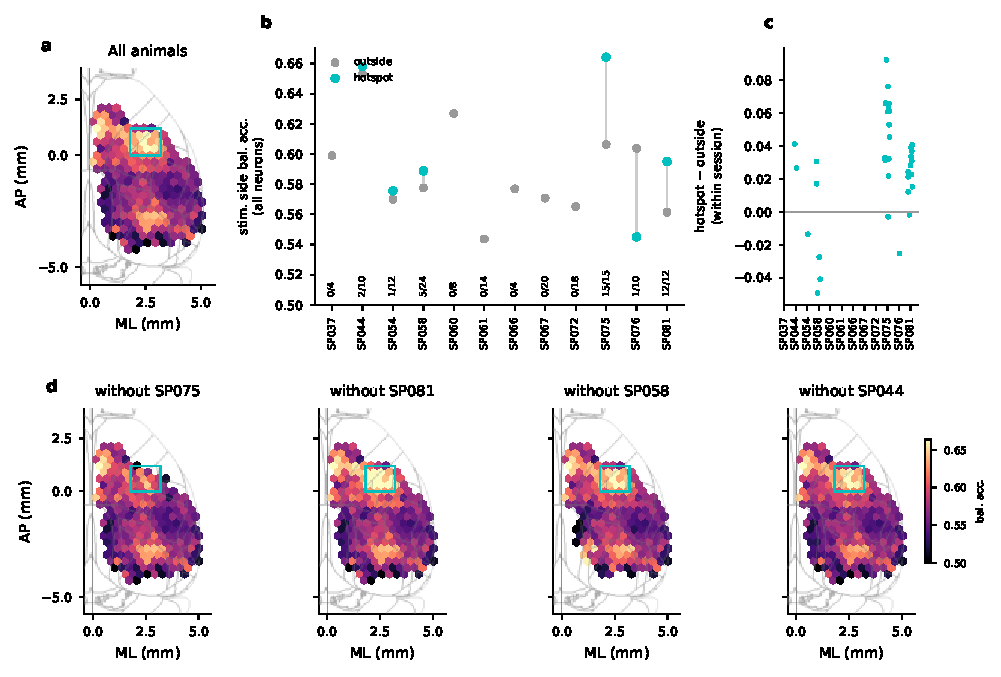
\includegraphics[width=7.00in,height=0.78\textheight,keepaspectratio]{si/si_stim_hotspot_panels.pdf}
  \caption{Is the mesoscope stimulus-side hotspot in SSp-ul / lateral MOp driven by single animals? 6 of 12 mice have sessions there, but 75\,\% of the hotspot sessions come from two mice, SP075 (15 sessions), SP081 (12 sessions). Mean score inside vs outside: 0.639 vs 0.580; without SP075: 0.596 vs 0.578; without SP081: 0.659 vs 0.582. Within sessions, the hotspot bins score +0.028 above the other bins on average (36 sessions; -0.005 without the two mice). Fraction of neurons tuned to stimulus side inside vs outside: 0.222 vs 0.143; without the two mice 0.095 vs 0.142. \textbf{a} Mesoscope stimulus-side decoding (all neurons of a session in a bin, mean over sessions; 0.4\,mm bins) with the hotspot region (cyan; bin centres ML 1.8--3.2\,mm, AP 0--1.2\,mm; mostly SSp-ul and MOp). \textbf{b} Per animal: mean score of the session $\times$ bin decoders inside (cyan) and outside (grey) the hotspot. Numbers: sessions with hotspot bins / all sessions of that animal. \textbf{c} Within-session contrast: for sessions with bins both inside and outside the hotspot, mean score inside minus outside. \textbf{d} Maps leaving out one animal (the four animals with most hotspot sessions; same colour scale as a).}
  \label{fig:si_stim_hotspot}
\end{figure}
